\documentclass{article}
\usepackage[utf8]{inputenc}
\usepackage[a4paper, total={6in, 9.5in}]{geometry}
\usepackage{amsmath}
\usepackage{amssymb}
\usepackage{minted}
\usepackage{graphicx}

\usepackage{tikz} % Import the tikz package
\usetikzlibrary{automata} % Import library for drawing automata
\usetikzlibrary{positioning} % ...positioning nodes
\usetikzlibrary{arrows} % ...customizing arrows
\tikzset{node distance=5cm, % Minimum distance between two nodes. Change if necessary.
every state/.style=
    { % Sets the properties for each state
        thick,
        fill=gray!10
    },
    initial text={}, % No label on start arrow
    double distance=2pt, % Adjust appearance of accept states
    every edge/.style={ % Sets the properties for each transition
        draw,
        ->,>=stealth', % Makes edges directed with bold arrowheads
        auto,
        semithick
    }
}
\let\epsilon\varepsilon

\title{Sheet 11}
\author{Digdarshan Kunwar}
\date{December 2018}
\begin{document}
\maketitle

\section*{Problem 11.1}
\subsection*{a)}
The definition of finite state machine \\
Here,\\
$FSM \ \left(\sum,S,s_{o},\delta,F \right)$\\
\\
$\sum = \{a,b\}$ \\ 
\textbf{S}=\{$S_{o},S_{1},S_{2}$\} \\ 
$\text{\textbf{s}}_{\textbf{0}}=\{S_{o}\} \\ 
\textbf{F}=\{S_{1}\}$\\ 
\begin{align*}
    \delta=\{ ((S_{o},b),S_{1}),(S_{o},a),S_{2}), \\
               (S_{1},a),S_{o}),(S_{1},b),S_{1}), \\
               (S_{2},a),S_{2}),(S_{2},b),S_{2})  \}
\end{align*}
\subsection*{b)}

\begin{center}
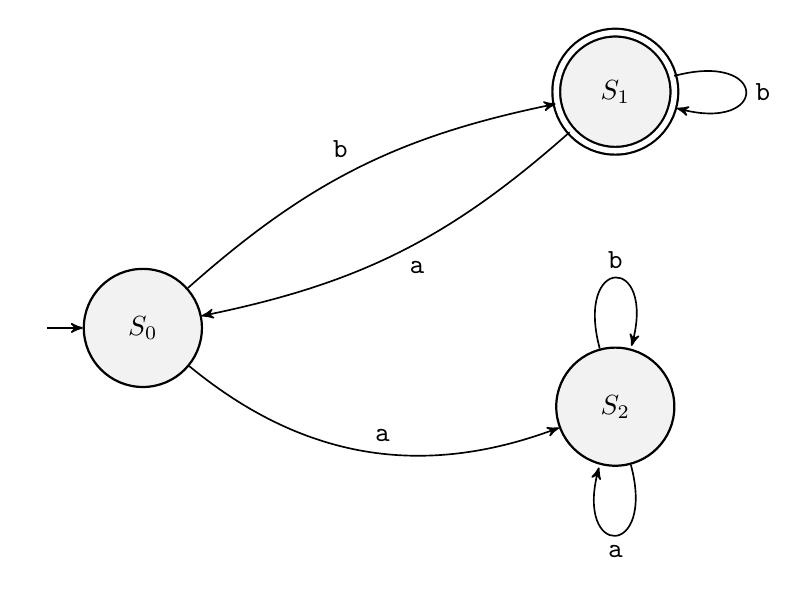
\begin{tikzpicture}
    \node[state, initial,minimum size=1.5cm] (1) at (0,0) {$S_{0}$};
    \node[state, accepting,minimum size=1.5cm] (2) at (6,3) {$S_{1}$};
    \node[state, minimum size=1.5cm] (3) at (6,-1) {$S_{2}$};
    \draw 
    (1) edge[bend left=15] node{\tt b} (2)
    (2) edge[bend left=15] node{\tt a} (1)
    (2) edge[loop right] node {\tt b}  (1)
    (1) edge[bend right] node{\tt a} (3)
    (3) edge[loop above] node{\tt b} (3)
    (3) edge[loop below] node{\tt a} (3)
    ;
\end{tikzpicture}
\end{center}
\subsection*{c)}
\begin{minted}{Haskell}
{-
CH08-320101_f2018
Problem 11.1 c) hs
Digdarshan Kunwar
d.kunwar@jacobs-university.de
-}
{-
Using results from HomeWork We can construct the following program
-}

data State = S0 | S1 | S2 | S3

accepts :: State -> String -> Bool

{-these are the equavalent delta functions from the documentation of the FSM-}
accepts S0 ('b':xs) = accepts S1 xs
accepts S0 ('a':xs) = accepts S2 xs
accepts S1 ('b':xs) = accepts S1 xs
accepts S1 ('a':xs) = accepts S0 xs
accepts S2 ('a':xs) = accepts S2 xs
accepts S2 ('b':xs) = accepts S2 xs


accepts S1 [] = True
accepts _ _ = False

fsm :: String -> Bool

{-Inital State-}
fsm = accepts S0

\end{minted}

\subsection*{d)}
Here:\\
Grammar required to generate the given set of rules:\\\\
$ \ \left(N,\sum,P,S\right)$\\
\\
$\sum = \{a,b\}$ \\ 
$N={S,T,U}$\\
$P=\{ S \rightarrow bT,T \rightarrow bT,T \rightarrow aX,X \rightarrow bT,X \rightarrow b, T \rightarrow \epsilon \}$\\\\
%%%%%%%%%%%%%%%%%%%%%%%%%%%%%%%%%%%%%%%%%%%%%%%%%%%%%%%%%%
\hline 
\text{   }\\
\section*{Problem 11.2 }
\subsection*{a)}
Initially \\
where x can be 0 or 1 \\\\
\begin{tabular}{|c|c|c|c|c|c|}
     $\downarrow$\\
     \hline
     \$ & 0 & x & x & x &\$  \\
     \hline
\end{tabular}\\\\
Here the logic is simple the machine initially starts at the first with the pointer(head) at \textbf{\$} so it moves right until it reaches a the ending \textbf{\$} that is at the rightmost part of the Turing tape.\\
So when the (head)pointer reads \textbf{\$} then it moves left and checks if the digit is 1 or 0.\\
If the digit is 0 then it rewrites it to 1 and moves to accepting(Final) state.\\
If the digit is 1 then it rewrites it to 0 and moves left and to the same state.So the pointer(head) moves left changing 1 to 0 until the head reads 0.\\

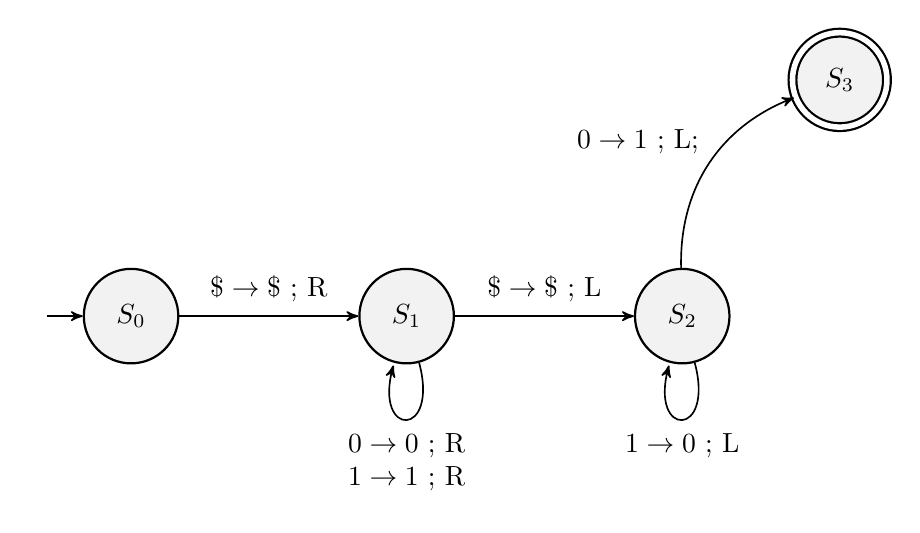
\begin{tikzpicture}
\node [state,initial,minimum size=1.2cm](1) at (0,0) {$S_{0}$};
\node [state,minimum size=1.2cm]        (2) at (3.5,0) {$S_{1}$};
\node [state,minimum size=1.2cm]        (3) at (7,0) {$S_{2}$};
\node [state,minimum size=1.2cm,accepting]       (4) at (9,3) {$S_{3}$};

\draw
    (1) edge node{
    \begin{tabular}{c}
            $\$\rightarrow \$$ ; R\\
    \end{tabular}
    } (2)
    
    (2) edge node{
    \begin{tabular}{c}
        $\$\rightarrow \$$ ; L\\
    \end{tabular}    
    } (3)
    
    (2) edge[loop below] node{
    \begin{tabular}{c}
       $0\rightarrow 0$ ; R \\
        $1\rightarrow 1$ ; R\\
    \end{tabular}    
    } (2)
    
    
    (3) edge[loop below] node{
    \begin{tabular}{c}
        $1\rightarrow 0$ ; L\\
    \end{tabular}    
    } (3)
    
    (3) edge[bend left=35] node {$0\rightarrow 1 $ ; L;} (4);
\end{tikzpicture}

%%%%%%%%%%%%%%%%%%%%%%%%%%%%%%%%%%%%%%%%%%%%%%%%%%%%%%%%%
\subsection*{b)}
Initially \\
where x can be 0 or 1 \\\\
\begin{tabular}{|c|c|c|c|c|c|}
     $\downarrow$\\
     \hline
     \$ & 0 & x & x & x &\$  \\
     \hline
\end{tabular}
\\\\\\
The logic is similar as that of question \textbf{a)} but in its initial movement form the leftmost \textbf{\$} to the rightmost \textbf{\$} the digits on the Turing tape are flipped (1 to 0 and 0 to 1).\\
So it adds one to the binary number and reaches state 3.\\
So after adding one,all the bits need to be flipped again.So the head moves to the right most \textbf{\$} and start flipping the digits (1 to 0 and 0 to 1) to it's way to the leftmost \textbf{\$} by moving left everytime until \textbf{\$} in the leftmost side is reached. 

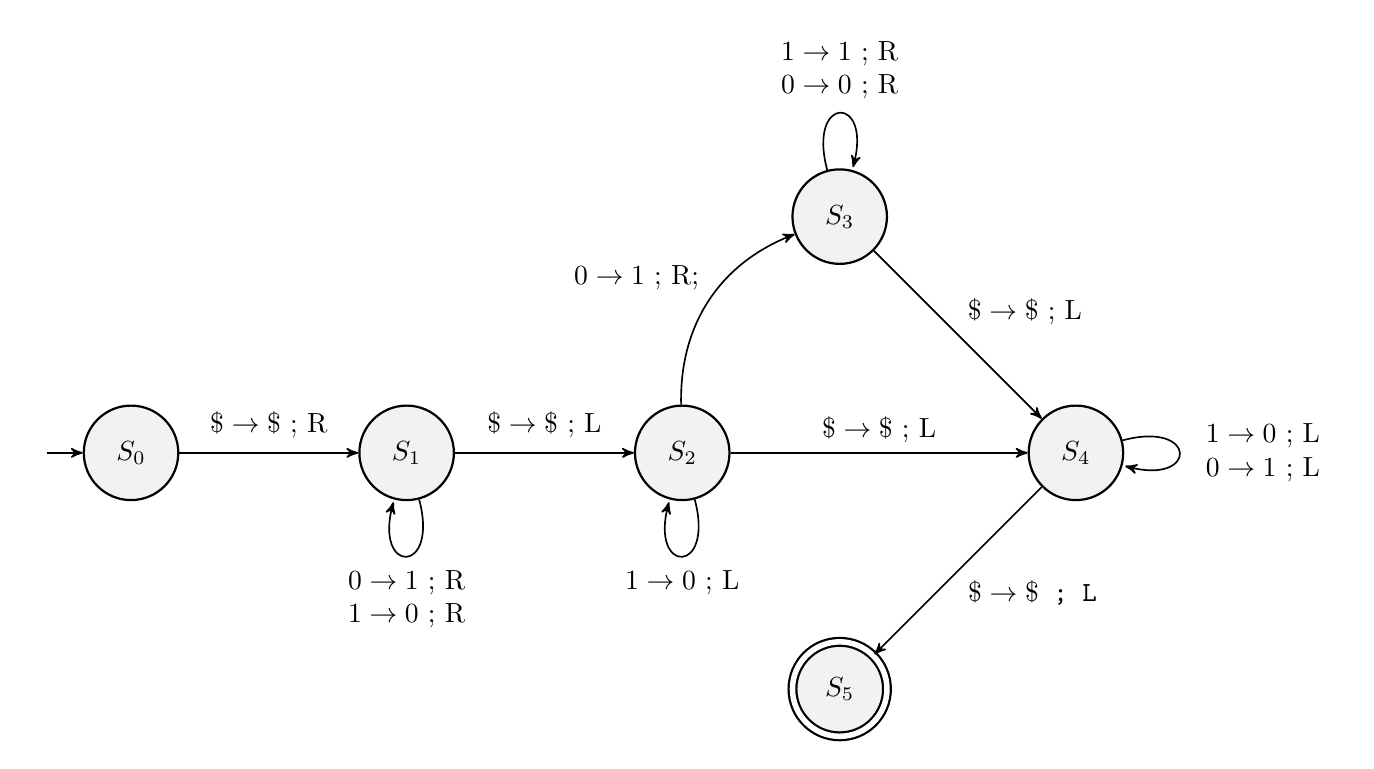
\begin{tikzpicture}
\node [state,initial,minimum size=1.2cm](1) at (0,0) {$S_{0}$};
\node [state,minimum size=1.2cm]        (2) at (3.5,0) {$S_{1}$};
\node [state,minimum size=1.2cm]        (3) at (7,0) {$S_{2}$};
\node [state,minimum size=1.2cm]       (4) at (9,3) {$S_{3}$};
\node [state,minimum size=1.2cm]       (5) at (12,0) {$S_{4}$};
\node [state,minimum size=1.2cm,accepting]       (6) at (9,-3) {$S_{5}$};

\draw
    (1) edge node{
    \begin{tabular}{c}
            $\$\rightarrow \$$ ; R\\
    \end{tabular}
    } (2)
    
    (2) edge node{
    \begin{tabular}{c}
        $\$\rightarrow \$$ ; L\\
    \end{tabular}    
    } (3)
    
    (2) edge[loop below] node{
    \begin{tabular}{c}
       $0\rightarrow 1$ ; R \\
        $1\rightarrow 0$ ; R\\
    \end{tabular}    
    } (2)
    
    (3) edge node{$\$\rightarrow \$ $ ; L } (5)
    
    (3) edge[loop below] node{
    \begin{tabular}{c}
        $1\rightarrow 0$ ; L\\
    \end{tabular}    
    } (3)
    
    (3) edge[bend left=35] node {$0\rightarrow 1 $ ; R;} (4)
    
    (4) edge[loop above] node {
    \begin{tabular}{c}
       $1\rightarrow 1$ ; R \\
        $0\rightarrow 0$ ; R\\
    \end{tabular}  
    } (4)
    
    (4) edge node{$\$\rightarrow \$ $ ; L } (5)
    (5) edge[loop right] node{
        \begin{tabular}{c}
        $1\rightarrow 0$ ; L \\
        $0\rightarrow 1$ ; L\\
         \end{tabular}
    } (5)
    (5) edge node{\tt $\$\rightarrow \$ $ ; L  } (6)
    
    ;
\end{tikzpicture}

\subsection*{\textbf{c)}}
Initially \\
where x can be 0 or 1 \\\\
\begin{tabular}{c c c c c c c c c c c}
     $T_{Add}$\\ $\downarrow$&&&&&&&&&&\\
     \hline
     \textbf{\$} & x & x & x & x &\textbf{\$} & x & x & x & x &\textbf{\$}  \\
     \hline\\
\end{tabular}\\
Here,\\
The logic is that once the number in the left part  decreases then the process starts to increase the number by one in the second part.\\
So every time until the binary number between the first \$ x x x x\$ are not \$0 0 0 0 \$ the Turing machine continuously decreases 1 to the first side and increases 1 to the second side.\\
So the final state is reached when all the digits in the left side are \$0 0 0 0 \$.\\
Until then the loop runs substrating one from the first part and adding one in the second.\\
So we combine the turing machine in \textbf{a)} and \textbf{b)}.

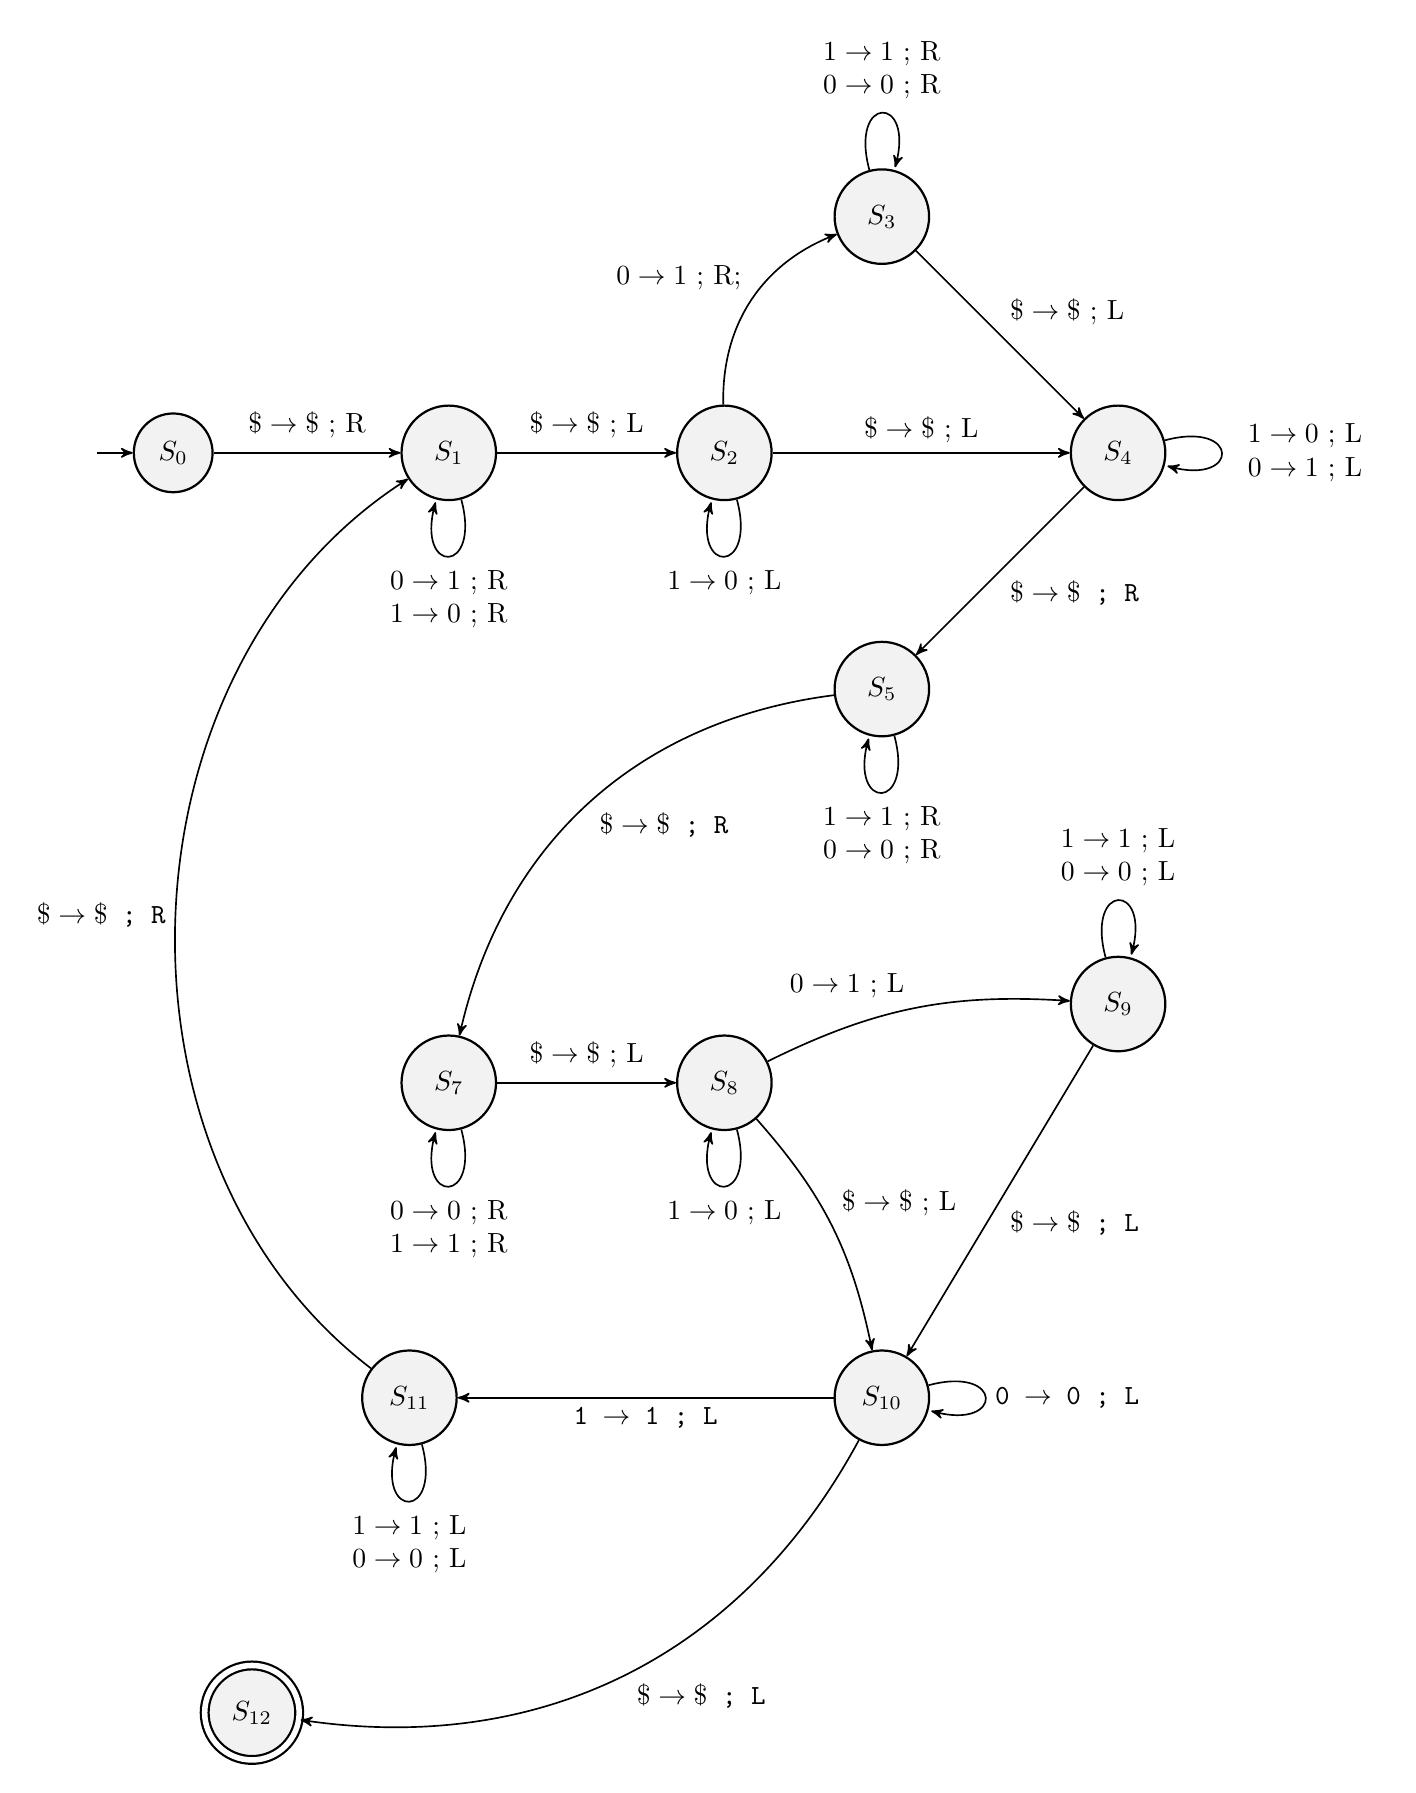
\begin{tikzpicture}
\node [state,initial,minimum size=1cm](1) at (0,0) {$S_{0}$};
\node [state,minimum size=1.2cm]        (2) at (3.5,0) {$S_{1}$};
\node [state,minimum size=1.2cm]        (3) at (7,0) {$S_{2}$};
\node [state,minimum size=1.2cm]       (4) at (9,3) {$S_{3}$};
\node [state,minimum size=1.2cm]       (5) at (12,0) {$S_{4}$};
\node [state,minimum size=1.2cm]       (6) at (9,-3) {$S_{5}$};
%%%%%%%%%%%%%%%%%%%%%%%%%%%%%%%%%%
%\node [state,minimum size=1.2cm](7) at (3,-4) {$S_{6}$};
\node [state,minimum size=1.2cm]        (8) at (3.5,-8) {$S_{7}$};
\node [state,minimum size=1.2cm]        (9) at (7,-8) {$S_{8}$};
\node [state,minimum size=1.2cm]       (10) at (12,-7) {$S_{9}$};
\node [state,minimum size=1.2cm]       (11) at (9,-12) {$S_{10}$};
\node [state,minimum size=1.2cm]       (12) at (3,-12) {$S_{11}$};
\node [state,minimum size=1.2cm,accepting]       (13) at (1,-16) {$S_{12}$};




\draw
    (1) edge node{
    \begin{tabular}{c}
            $\$\rightarrow \$$ ; R\\
    \end{tabular}
    } (2)
    
    (2) edge node{
    \begin{tabular}{c}
        $\$\rightarrow \$$ ; L\\
    \end{tabular}    
    } (3)
    
    (2) edge[loop below] node{
    \begin{tabular}{c}
       $0\rightarrow 1$ ; R \\
        $1\rightarrow 0$ ; R\\
    \end{tabular}    
    } (2)
    
    (3) edge node{$\$\rightarrow \$ $ ; L } (5)
    
    (3) edge[loop below] node{
    \begin{tabular}{c}
        $1\rightarrow 0$ ; L\\
    \end{tabular}    
    } (3)
    
    (3) edge[bend left=35] node {$0\rightarrow 1 $ ; R;} (4)
    
    (4) edge[loop above] node {
    \begin{tabular}{c}
       $1\rightarrow 1$ ; R \\
        $0\rightarrow 0$ ; R\\
    \end{tabular}  
    } (4)
    
    (4) edge node{$\$\rightarrow \$ $ ; L } (5)
    (5) edge[loop right] node{
        \begin{tabular}{c}
        $1\rightarrow 0$ ; L \\
        $0\rightarrow 1$ ; L\\
         \end{tabular}
    } (5)
    (5) edge node{\tt $\$\rightarrow \$ $ ; R  } (6)
    
    (6) edge[loop below] node {
    \begin{tabular}{c}
       $1\rightarrow 1$ ; R \\
        $0\rightarrow 0$ ; R\\
    \end{tabular}  
    } (6)
    
    
    (6) edge[bend right=35] node{\tt $\$\rightarrow \$$ ; R\\ }(8)
%%%%%%%%%%%%%%%%%%%%%%%%%%%%%%%%%%%%%%%%%%%%%%%
    (8) edge node{
    \begin{tabular}{c}
        $\$\rightarrow \$$ ; L\\
    \end{tabular}    
    } (9)
    
    (8) edge[loop below] node{
    \begin{tabular}{c}
       $0\rightarrow 0$ ; R \\
        $1\rightarrow 1$ ; R\\
    \end{tabular}    
    } (8)
    
    
    (9) edge[loop below] node{
    \begin{tabular}{c}
        $1\rightarrow 0$ ; L\\
    \end{tabular}    
    } (9)
    
    (9) edge[bend left=15] node {$0\rightarrow 1 $ ; L} (10)
    (9) edge[bend left=15] node {$\$ \rightarrow \$ $ ; L} (11)
    
    (10) edge[loop above] node {
    \begin{tabular}{c}
       $1\rightarrow 1$ ; L \\
        $0\rightarrow 0$ ; L\\
    \end{tabular}  
    } (10)
    
    (10) edge node{\tt $\$\rightarrow \$$ ; L\\} (11)
    (11) edge node{\tt  1 $\rightarrow $ 1 ; L\\} (12)
    (11) edge[loop right] node{\tt  0 $\rightarrow $ 0 ; L\\} (11)
    (11) edge[bend left=35] node{\tt   $\$ \rightarrow \$ $ ; L\\} (13)
    (12) edge[bend left=55] node{\tt   $\$ \rightarrow \$ $ ; R\\} (2)
    
    (12) edge[loop below] node {
    \begin{tabular}{c}
       $1\rightarrow 1$ ; L \\
        $0\rightarrow 0$ ; L\\
    \end{tabular}  
    } (12)
    
    ;
\end{tikzpicture}
\end{document}
